
\begin{frame}{Content}{}
\tableofcontents
\end{frame}

%-------------------------------------------------------
%-------------------------------------------------------
\section{Introduction}
%-------------------------------------------------------
%-------------------------------------------------------
%%%%%%%%%%%%%%%%%%%%%%%%%%%%%
%         SLIDE             %
%%%%%%%%%%%%%%%%%%%%%%%%%%%%%
\begin{frame}
  \frametitle{Particle physics: today and future}

  \begin{itemize}
  \item The Large Hadron Collider (LHC) is today's largest particle
    accelerator at CERN (European Organisation for Nuclear Research)
    \begin{itemize}
    \item Proton-proton collisions
    \item Center-of-mass energy: $\sqrt{s}=13\,\tev$
    \item Observation of the Higgs boson in 2012
    \end{itemize}

  \item Still open questions in particles physics remain unanswered:
    \begin{itemize}
    \item Full understanding of the Higgs boson
    \item The origin of matter-antimatter asymmetry
    \item Dark matter
    \item Many more questions ...
    \end{itemize}

  \item Several approaches of high-energy particle colliders to
    address the unanswered questions in the post-LHC era:
    \begin{itemize}
    \item proton-proton ($p~p$) colliders
      \\
      \textcolor{Red}{and/or}
      \\
    \item electron-positron ($e^+e^-$) colliders
    \end{itemize}
  \end{itemize}

\end{frame}

%%%%%%%%%%%%%%%%%%%%%%%%%%%%%
%         SLIDE             %
%%%%%%%%%%%%%%%%%%%%%%%%%%%%%
\begin{frame}
  \frametitle{Hadron vs. Lepton colliders $\Rightarrow$ Discovery to Precision}
  
  % \begin{block}{}
  %   \centering
  %   Discovery to Precision
  % \end{block}

  \begin{columns}[t]
    \column{0.5\textwidth}
    \centering
    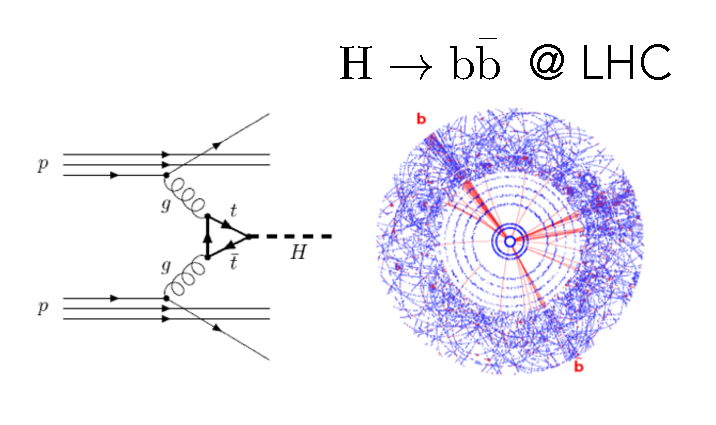
\includegraphics[width=0.6\textwidth]{figures/hadronColliders.pdf}

    \column{0.5\textwidth}
    \centering
    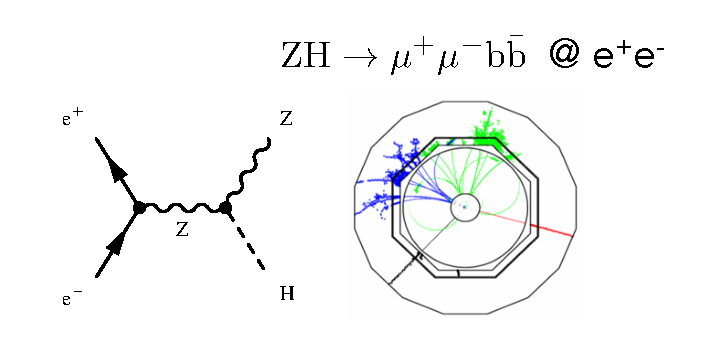
\includegraphics[width=0.6\textwidth]{figures/leptonColliders.pdf}

  \end{columns}


  \begin{columns}[t]
    \column{0.5\textwidth}

    \begin{itemize}
    \item Protons $\Rightarrow$ compound objects
      \begin{itemize}
      \item Unknown event-by-event initial states
      \item Limited achievable precision
      \end{itemize}
    \item High rates of QCD backgrounds
      \begin{itemize}
      \item Complex triggering schemes
      \item High levels of radiation
      \end{itemize}
    \item High cross-sections for coloured-states
    \item High-energy circular pp colliders are feasible
    \end{itemize}

    \column{0.5\textwidth}

    \begin{itemize}
    \item Electrons/positrons $\Rightarrow$ point like
      \begin{itemize}
      \item Well-defined initial states (energy, polarisation)
      \item High-precision measurements
      \end{itemize}
    \item Cleaner experimental environment
      \begin{itemize}
      \item Trigger-less readout
      \item Low levels of radiation
      \end{itemize}
    \item Superior sensitivity for electro-weak states
    \item High-energy $e^+e^-$ collisions ($\geq350\,\tev$) require
      linear colliders
    \end{itemize}

  \end{columns}

\end{frame}


%%%%%%%%%%%%%%%%%%%%%%%%%%%%%
%         SLIDE             %
%%%%%%%%%%%%%%%%%%%%%%%%%%%%%
\begin{frame}
  \frametitle{High-energy $e^+e^-$ colliders studies at CERN}

  \begin{columns}
    \column{0.6\textwidth}
    \begin{itemize}
    \item The Compact LInear Collider (CLIC)
      \begin{itemize}
      \item An $e^{+}e^{-}$ linear collider for the post HL-LHC period.
      \item Energy range $\sqrt{s}$ : \textcolor{blue}{$380\,\gev$} to
        \textcolor{blue}{$3\,\tev$}
        \begin{itemize} 
        \item Two-beam acceleration scheme with gradients of $\sim$100~MV/m.
        \end{itemize}
      \item Precision measurements of:
        \begin{itemize}
        \item Standard Model processes (Higgs, top).
        \item New physics potentially discovered at 13~TeV LHC.
        \item Search for new physics: unique sensitivity to particles with
          electroweak charge.
        \end{itemize}
      \end{itemize}
    \end{itemize}

    \column{0.4\textwidth}
    \begin{tikzpicture}
      \node[anchor=south west,inner sep=0] (image) at (0,
      0){\includegraphics[width=\textwidth]{../figures/CLIC/staging.pdf}};
      \begin{scope}[x={(image.south east)},y={(image.north west)}]
        \node[above, color=white] at (0.5, 0.001) {\textbf{48 km tunnel at 3 TeV stage}};
      \end{scope}
    \end{tikzpicture}
  \end{columns}
  
  \begin{columns}
    \column{0.7\textwidth}

    \begin{itemize}
    \item The Future Circular Collider (FCC-ee):
      \begin{itemize}
      \item Lepton collider in a new 80-100~km tunnel around CERN.
      \item Energy range $\sqrt{s}$: from $90\,\gev$ to $350\,\gev$.
      \item FCC-hh: for proton-proton collisions $\sqrt{s}$ is up to $100\,\tev$.
      \end{itemize}
    \end{itemize}

    \column{0.3\textwidth}
    \centering
    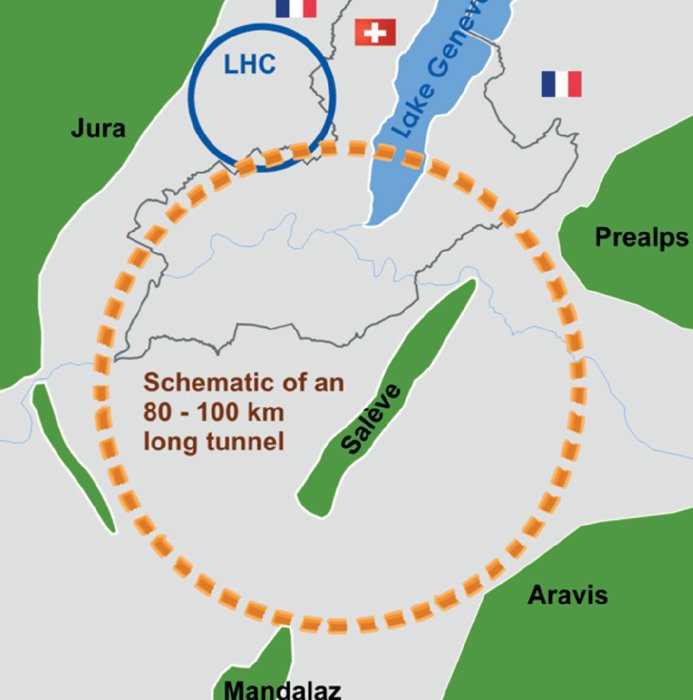
\includegraphics[width=0.9\textwidth]{figures/FCC}

  \end{columns}

\end{frame}


%%%%%%%%%%%%%%%%%%%%%%%%%%%%%
%         SLIDE             %
%%%%%%%%%%%%%%%%%%%%%%%%%%%%%
{
  \usebackgroundtemplate{
    \begin{picture}(100, 265)
      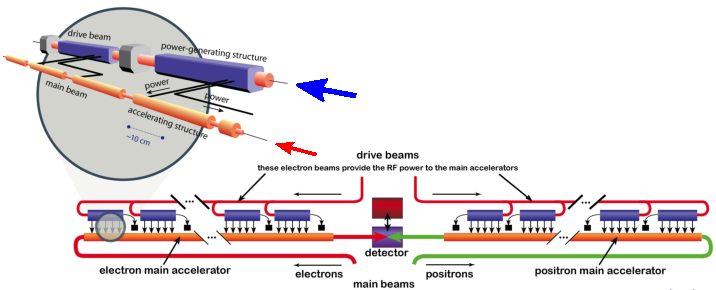
\includegraphics[width=\textwidth]{figures/CLIC_2beam_accel.pdf}
    \end{picture}
  }%
  \begin{frame}
    \frametitle{Two-beam acceleration scheme at CLIC}
    
    \vspace{-1.8cm}
    \begin{itemize}
    \item High-gradient acceleration of \textcolor{Red}{100~MV/m} at
      \textcolor{Red}{12~GHz} \\
      ($\rightarrow$ LHC: 5~MV/m and 400~MHz)
      \begin{itemize}
      \item Limit the length of the accelerator
      \item Traditional klystrons ($\sim$1~GHz) accelerate the drive
        beam (low energy \& high intensity)
      \item Drive beam decelerated $\rightarrow$ energy is fed via an
        RF field in a waveguide to the main beam.
      \end{itemize}
    \end{itemize}
    
    \begin{columns}
      \column{0.5\textwidth}
      \column{0.5\textwidth}
      \begin{itemize}
      \item \textcolor{blue}{Drive beam $\Rightarrow$ RF power}
        \begin{itemize}
        \item 12~GHz bunch structure
        \item High current 100~A
        \item Low energy $2.4\,\gev$ - $240\,\gev$
        \end{itemize}
      \item \textcolor{red}{Main beam $\Rightarrow$ physics}
        \begin{itemize}
        \item Lower current 1.2~A
        \item High energy $9\,\gev$ - $1.5\,\tev$
        \end{itemize}
      \end{itemize}
    \end{columns}

  \end{frame}
}

%%%%%%%%%%%%%%%%%%%%%%%%%%%%%
%         SLIDE             %
%%%%%%%%%%%%%%%%%%%%%%%%%%%%%
\subsection{CLIC beam profile}
\begin{frame}
  \frametitle{Beam profile for CLIC}

 \begin{columns}
   \column{0.6\textwidth}

   \begin{itemize}
   \item Limited train duration due to the duration of the high power levels.
     \begin{itemize}
     \item Bunch crossings (BX): every 0.5~ns.
     \item Train duration: 156~ns (312 bunches).
     \item Train repetition: 20~ms (50~Hz).
     \end{itemize}
   \end{itemize}

   \column{0.4\textwidth}
   \begin{tikzpicture}
     \node[anchor=south west,inner sep=0] (image) at (0,
     0){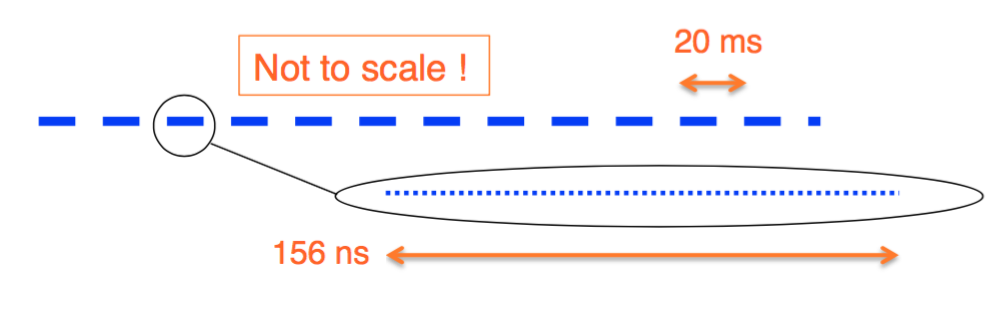
\includegraphics[width=\textwidth]{figures/CLICbeam.png}};
     \begin{scope}[x={(image.south east)},y={(image.north west)}]
       \node[above, color=blue] at (0.5, 0.9) {\textbf{CLIC bunch
           structure}};
     \end{scope}
   \end{tikzpicture}
 \end{columns}
 
 \centering
 \resizebox{0.9\columnwidth}{!}{\begin{tabular}{l c c} 
                                  \toprule 
                                  & CLIC at $\sqrt{s}=3\,\tev$ & LHC at $\sqrt{s}=13\,\tev$\\
                                  \midrule
                                  Instantaneous luminosity $\mathcal{L}$ & $6\times10^{34}$ \inversecmsquaredsec & $1\times10^{34}$ \inversecmsquaredsec \\
                                  Bunch-crossing separation & 0.5~ns & 25~ns \\
                                  IP size in x / y / z directions & 45~nm / 1~nm / $44\,\micron$ & $15\,\micron$ / $15\,\micron$ / 50~cm \\
                                  \bottomrule
                                \end{tabular}
}
                              
                              % \column{0.5\textwidth}
                              % \centering



\begin{itemize}
\item \textcolor{Red}{Bunch separation and train duration: drive
    timing resolution requirements for the detectors.}
\item \textcolor{Green}{Very small beam sizes at the interaction
    point} $\Rightarrow$ beam-induced backgrounds
\end{itemize}



\begin{itemize}
\item Short train duration implies:
  \begin{itemize}
  \item triggerless readout of the detectors.
  \item power pulsing: allows to reduce the average power dissipation.
  \end{itemize}
\end{itemize}

\end{frame}


%%%%%%%%%%%%%%%%%%%%%%%%%%%%%
%         SLIDE             %
%%%%%%%%%%%%%%%%%%%%%%%%%%%%%
\begin{frame}
  \frametitle{Beam-induced backgrounds}
  
  \begin{columns}
    \column{0.8\textwidth}
    \begin{itemize}
    \item Backgrounds:
      \begin{itemize}
      \item \textcolor{blue}{$e^{+}e^{-}$ pairs}: low $p_{T}$, forward
        peaked, limits the inner radius of the VXD.
      \item \textcolor{blue}{$\gamma\gamma\rightarrow$hadrons}: larger
        $p_{T}$ particles, main background in the calorimeters and
        trackers.
      \end{itemize}
    \end{itemize}
    
    \column{0.2\textwidth}    
    \centering
    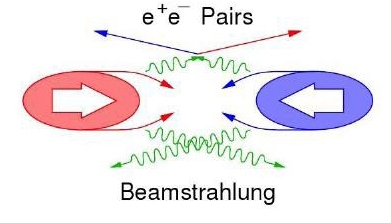
\includegraphics[width=\textwidth]{figures/beamstrahlung.png}
  \end{columns}

  \begin{columns}
    \column{.5\textwidth}    
    \begin{itemize}
    \item Each train consists of:
      \begin{itemize}
      \item At most 1 interesting event.
      \item $>$ 30000 background particles inside the detector.
      \end{itemize}
    \end{itemize}

    \column{0.5\textwidth}
    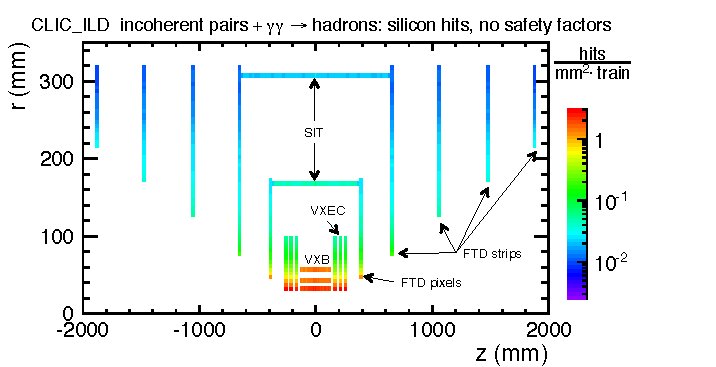
\includegraphics[width=\textwidth]{figures/background_vertex.pdf}
  \end{columns}

  \begin{itemize}
    % \item At most 1 interesting event in each train, $\approx$ 1000 hadronic background events are produced.
  \item Occupancy in the pixel detectors for each train (during \SI{156}{\nano\second}): $\sim$ 3\% for innermost layers.
  \item Radiation exposure of the vertex detector is moderate:
    \begin{itemize}
    \item Total ionising dose (TID): 200~Gy/yr
    \item Non-ionising energy loss (NIEL): $10^{11} n_{eq}/cm^{2}/yr$ (\textcolor{blue}{for ATLAS phase 1: $10^{15} n_{eq}/cm^{2}/yr$})
    \end{itemize}
  \end{itemize}

\end{frame}

%%%%%%%%%%%%%%%%%%%%%%%%%%%%%
%         SLIDE             %
%%%%%%%%%%%%%%%%%%%%%%%%%%%%%
\section{Requirements}
\begin{frame}
  \frametitle{The CLIC detector}

  \begin{columns}
    \column{0.5\textwidth}
    \begin{tikzpicture}
      \node[anchor=south west,inner sep=0] (image) at (0,
      0){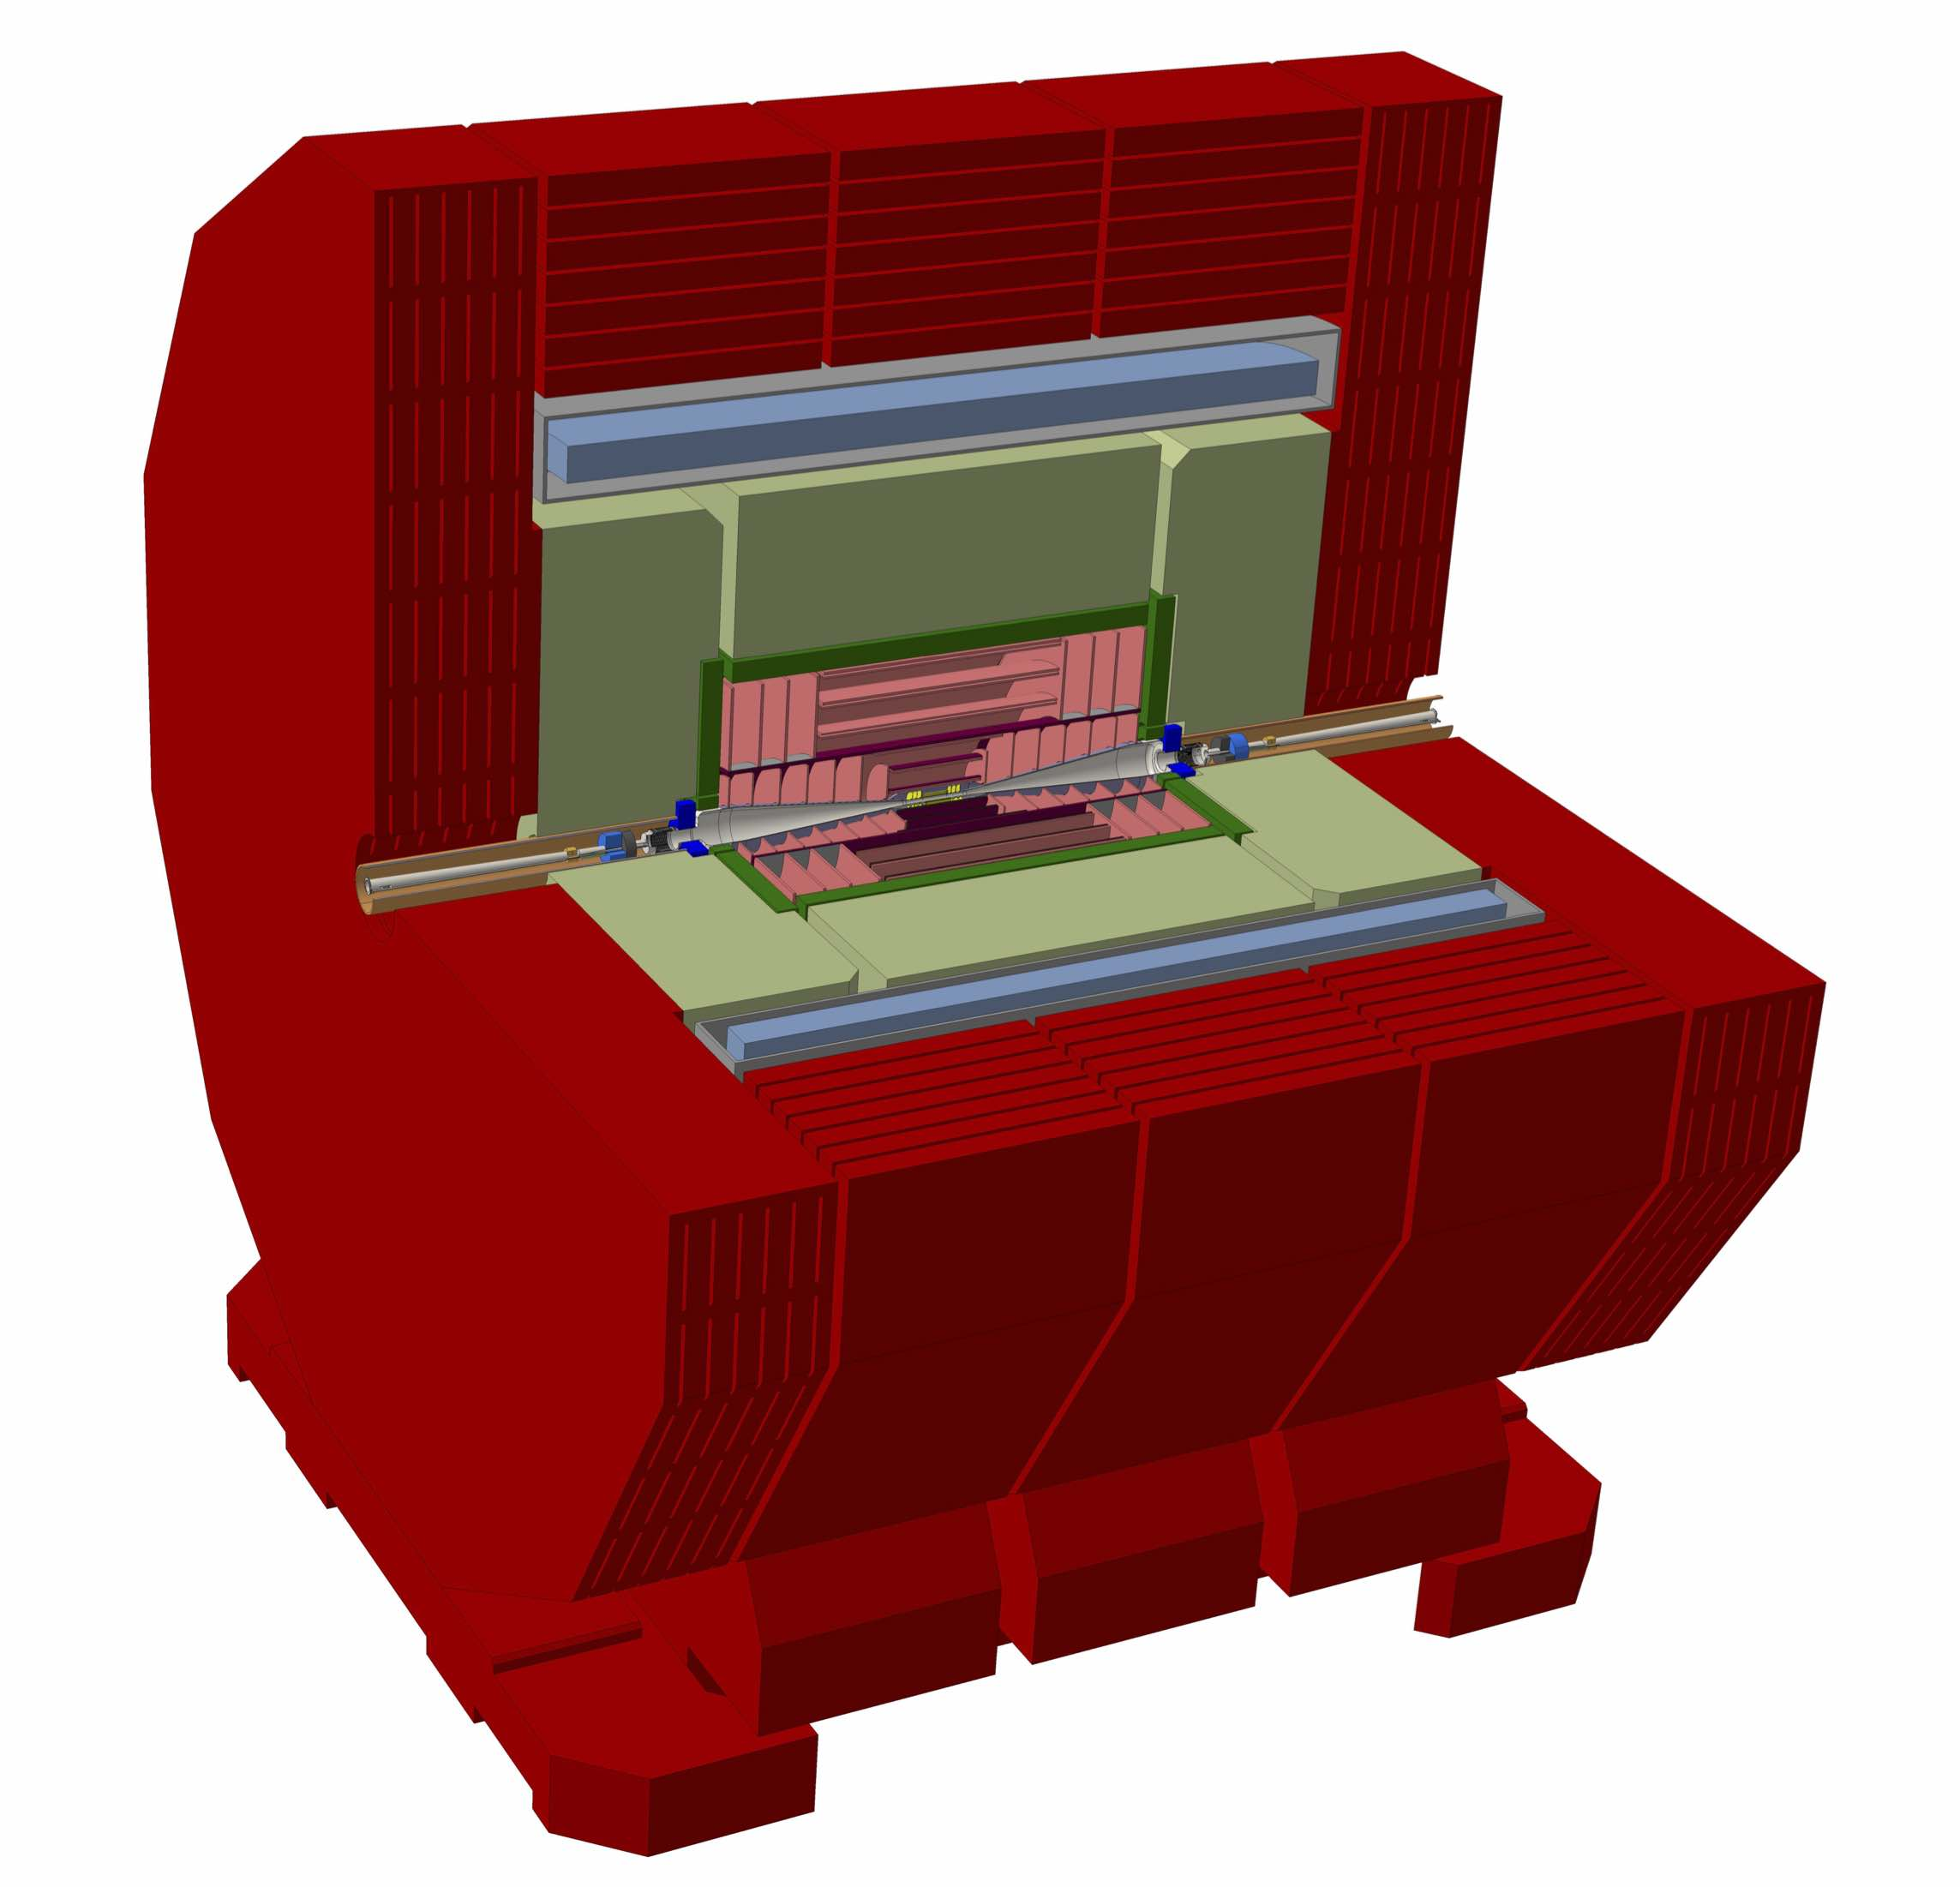
\includegraphics[width=\textwidth]{figures/CLIC_detector_2016.jpg}};
      \begin{scope}[x={(image.south east)},y={(image.north west)}]

        % \draw[help lines,xstep=.1,ystep=.1] (0, 0) grid (1,1);
        % \foreach \x in {0,1,...,9} { \node [anchor=north] at (\x/10,0) {0.\x}; }
        % \foreach \y in {0,1,...,9} { \node [anchor=east] at (0,\y/10)
        %   {0.\y}; }

        \draw[<->,line width=0.5pt] (0.32, 0.0) -- (0.8, 0.13);
        \node[color=black] at (0.6, 0.02) {11.4~m};

        \draw[<->,line width=0.5pt] (0.04, 0.17) -- (0.04, 0.9);
        \node[color=black, rotate=90] at (0.01, 0.5) {12.9~m};
      \end{scope}
    \end{tikzpicture}

    \column{0.5\textwidth}
    \begin{itemize}
    \item CMS-like detector (????? TO BE CHECKED)
    \item Silicon-based and low mass tracking system.
    \item Fine-grained calorimetry system (ECAL and HCAL) optimised
      for particle flow analysis (PFA).
    \item Superconducting solenoid magnet: B=4~T.
    \item Return iron yoke with detectors for muon identification.
    \item Forward region with LumiCal (luminosity monitoring) and
      BeamCal (beam calorimeter).
    \end{itemize}

  \end{columns}

\end{frame}

%%%%%%%%%%%%%%%%%%%%%%%%%%%%%
%         SLIDE             %
%%%%%%%%%%%%%%%%%%%%%%%%%%%%%
\begin{frame}
  \frametitle{Requirements for the vertex detector}

  \begin{columns}
    \column{0.75\textwidth}
    \begin{itemize}
    \item Efficient tagging of heavy quarks through a precise
      determination of displaced vertices can be achieved by: 
      \begin{itemize}
      \item Multi-layer VXD: 6 layers in the barrel and 6 disks
      \item B-field: \textcolor{Blue}{4~T}.
      \item Single point resolution of
        \textcolor{Blue}{$\sim$\SI{3}{\micro\meter}}:
        \textcolor{Blue}{\SI{25}{\micro\meter}} pixel pitch \& analog readout.
      \item Low material budget: $<0.2\%$~X\textsubscript{0}/layer and beam-pipe
        \begin{itemize}
        \item forced airflow cooling \& low-power electronics
          ($\approx 50$~mW/cm\textsuperscript{2})
        \end{itemize}
      \end{itemize} 
    \end{itemize}

    \column{0.25\textwidth}
    \centering
    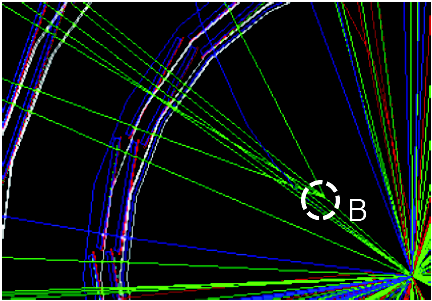
\includegraphics[width=\textwidth]{figures/secondary_vertex.png}

  \end{columns}

  \vspace{-0.3cm}  
  \begin{columns}
    \column{0.6\textwidth}
    \begin{itemize}
    \item Time slicing of \textcolor{Blue}{$\sim$\SI{10}{\nano\second}}
      to reduce the impact of beam-induced backgrounds. \\
      $\Rightarrow$ high-resistive \& depleted sensors, readout with precise timing.
    \end{itemize}

    \column{0.4\textwidth}
    \centering
    \begin{tikzpicture}
      \node[anchor=south west,inner sep=0] (image) at (0,
      0){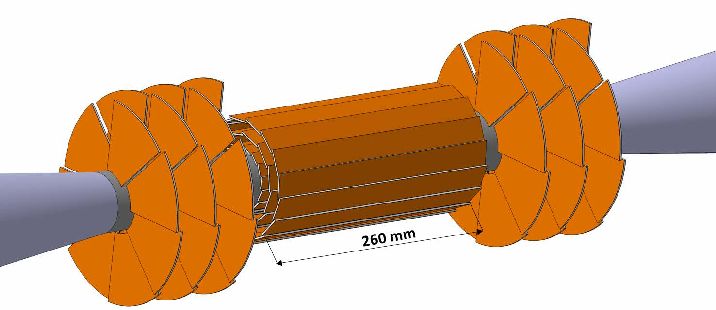
\includegraphics[width=\textwidth]{figures/spiralVXD.pdf}};
      \begin{scope}[x={(image.south east)},y={(image.north west)}]
        \draw[<->, Blue, thick](0.2, 0.0)--(0.84, 0.2);
        \node[below, color=Blue] at (0.5, 0.05) {56 cm};

        % \draw[help lines,xstep=.1,ystep=.1] (0, 0) grid (1,1);
        % \foreach \x in {0,1,...,9} { \node [anchor=north] at (\x/10,0) {0.\x}; }
        % \foreach \y in {0,1,...,9} { \node [anchor=east] at (0,\y/10)
        %   {0.\y}; }

      \end{scope}
    \end{tikzpicture}
  \end{columns}

  % \begin{itemize}
  %   \item Moderate radiation exposure of the vertex detector:
  %     \begin{itemize}
  %     \item Total ionising dose (TID): $<$1~kGy/yr
  %     \item Non-ionising energy loss (NIEL): $10^{11}$~n\textsubscript{eq}/cm\textsuperscript{2}/yr (\textcolor{Blue}{ATLAS phase 1: $10^{15}$~n\textsubscript{eq}/cm\textsuperscript{2}/yr})
  %     \end{itemize}
  % %% \item Time slicing of \textcolor{Blue}{$\sim$\SI{10}{\nano\second}}
  % %%   to reduce the impact of beam-induced backgrounds. \\
  % %%   $\Rightarrow$ high-resistive \& depleted sensors, readout with precise timing.
  % \end{itemize}

\end{frame}

%%%%%%%%%%%%%%%%%%%%%%%%%%%%%
%         SLIDE             %
%%%%%%%%%%%%%%%%%%%%%%%%%%%%%
\begin{frame}
  \frametitle{Flavour-tagging at CLIC}

  \begin{columns}
    \column{0.6\textwidth}
    \begin{itemize}
    \item At $\sqrt{s}=3\,\tev$ the production of the $126\,\gev$
      Higgs
      boson is dominated by the process: \\
      e$^+$e$^- \rightarrow$H$\nu\bar{\nu}$
    \item The Higgs boson decays to b\={b} and c\={c} quark pairs.
    \end{itemize}

    \column{0.4\textwidth}
    \centering
    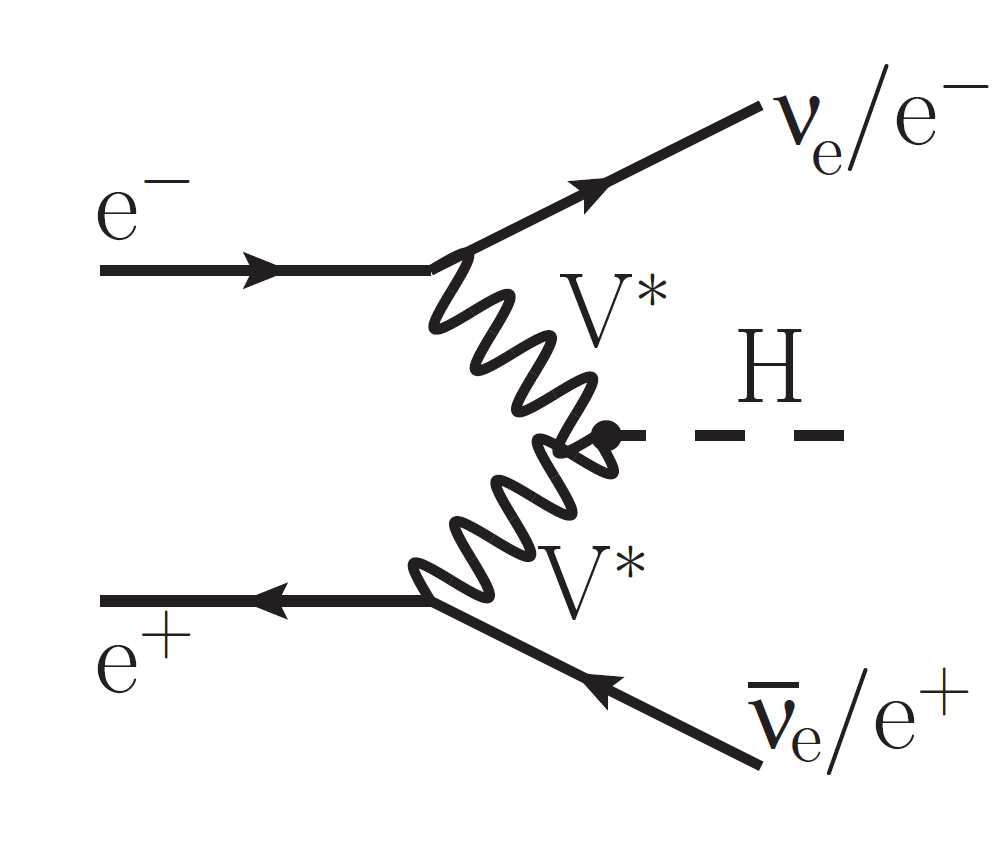
\includegraphics[width=0.5\textwidth]{figures/feynman_higgs.png}
  \end{columns}

  \begin{itemize}
  \item A high-precision vertex detector allows for beauty and
    charm-tagging and to study such decay modes.
  \end{itemize}

  \begin{columns}
    \column{0.5\textwidth}
    \centering
    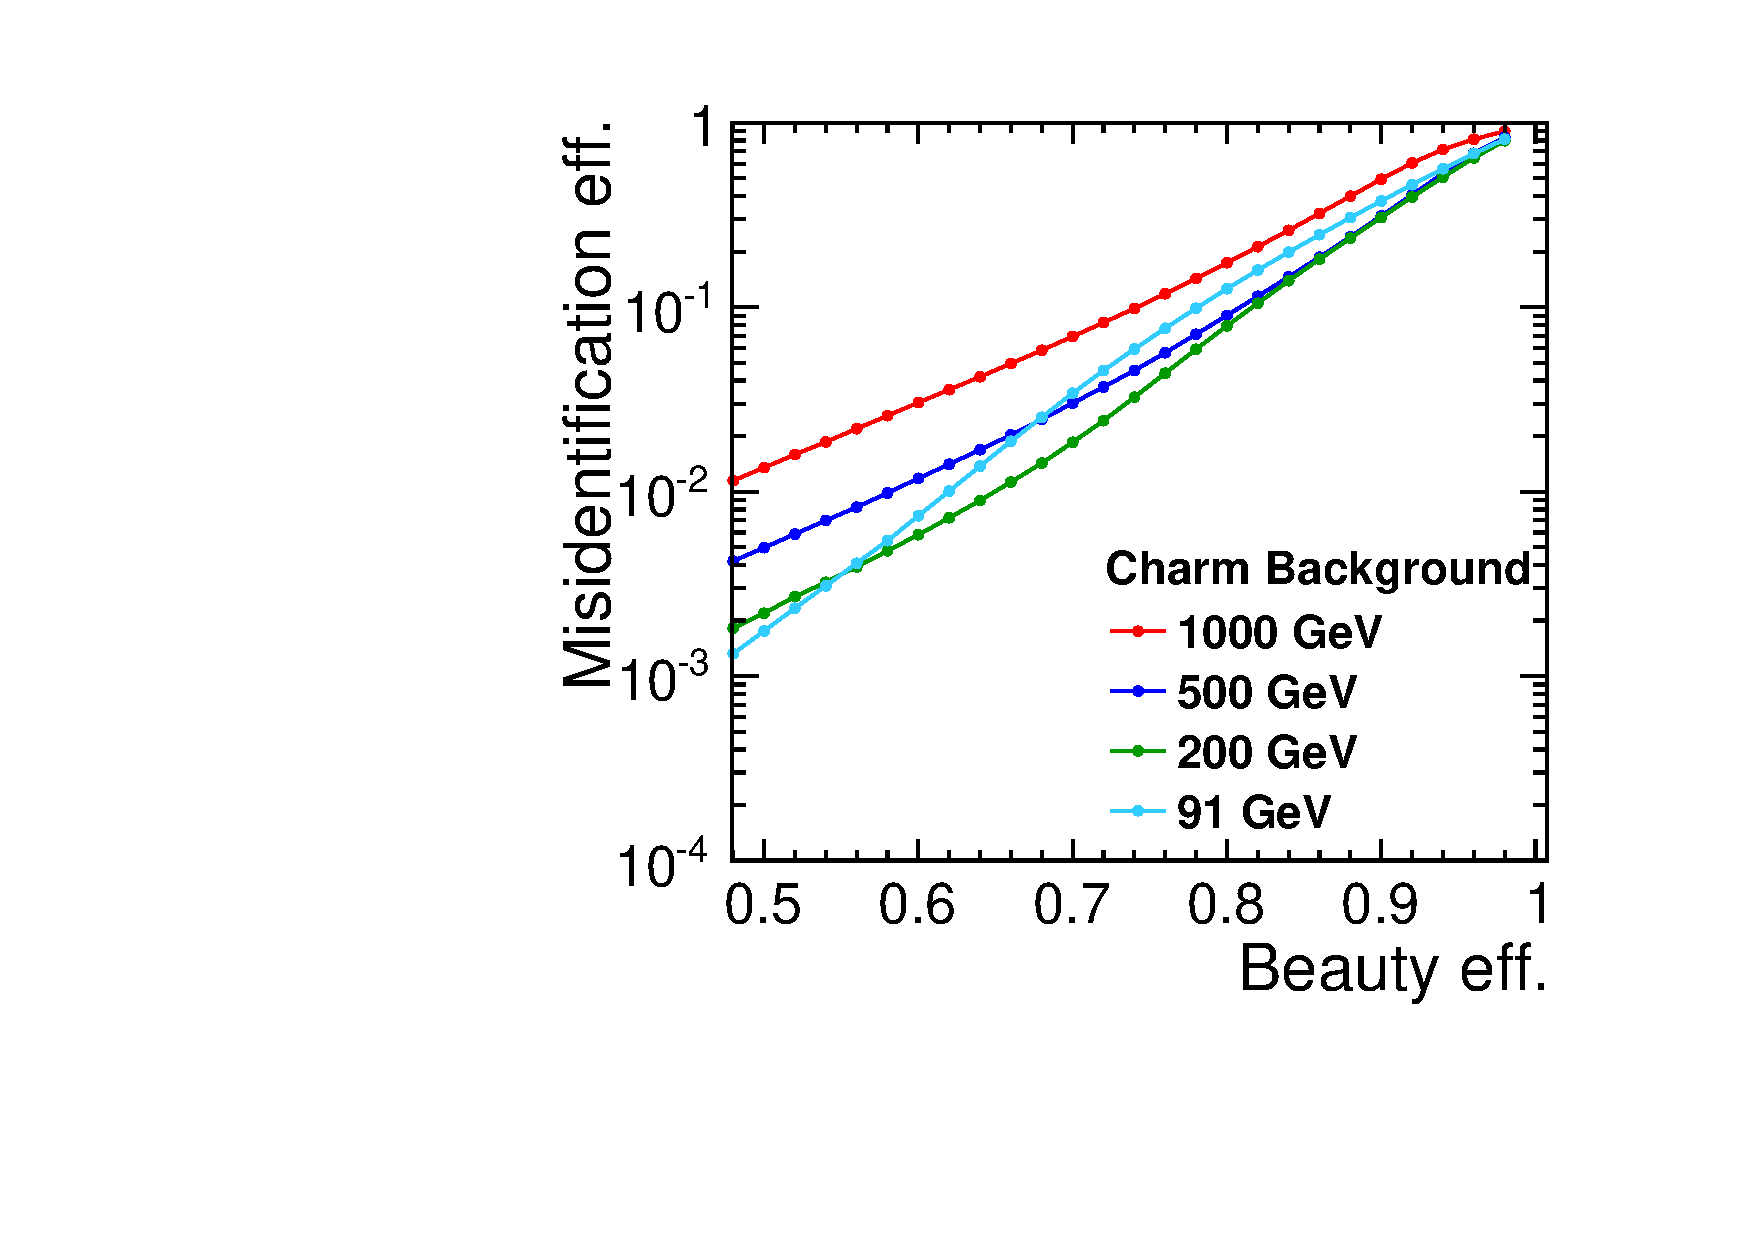
\includegraphics[width=\textwidth]{figures/Global_energies_CLIC_SiD_spirals_Beauty_Charm_.pdf}
    \column{0.5\textwidth}
    \centering
    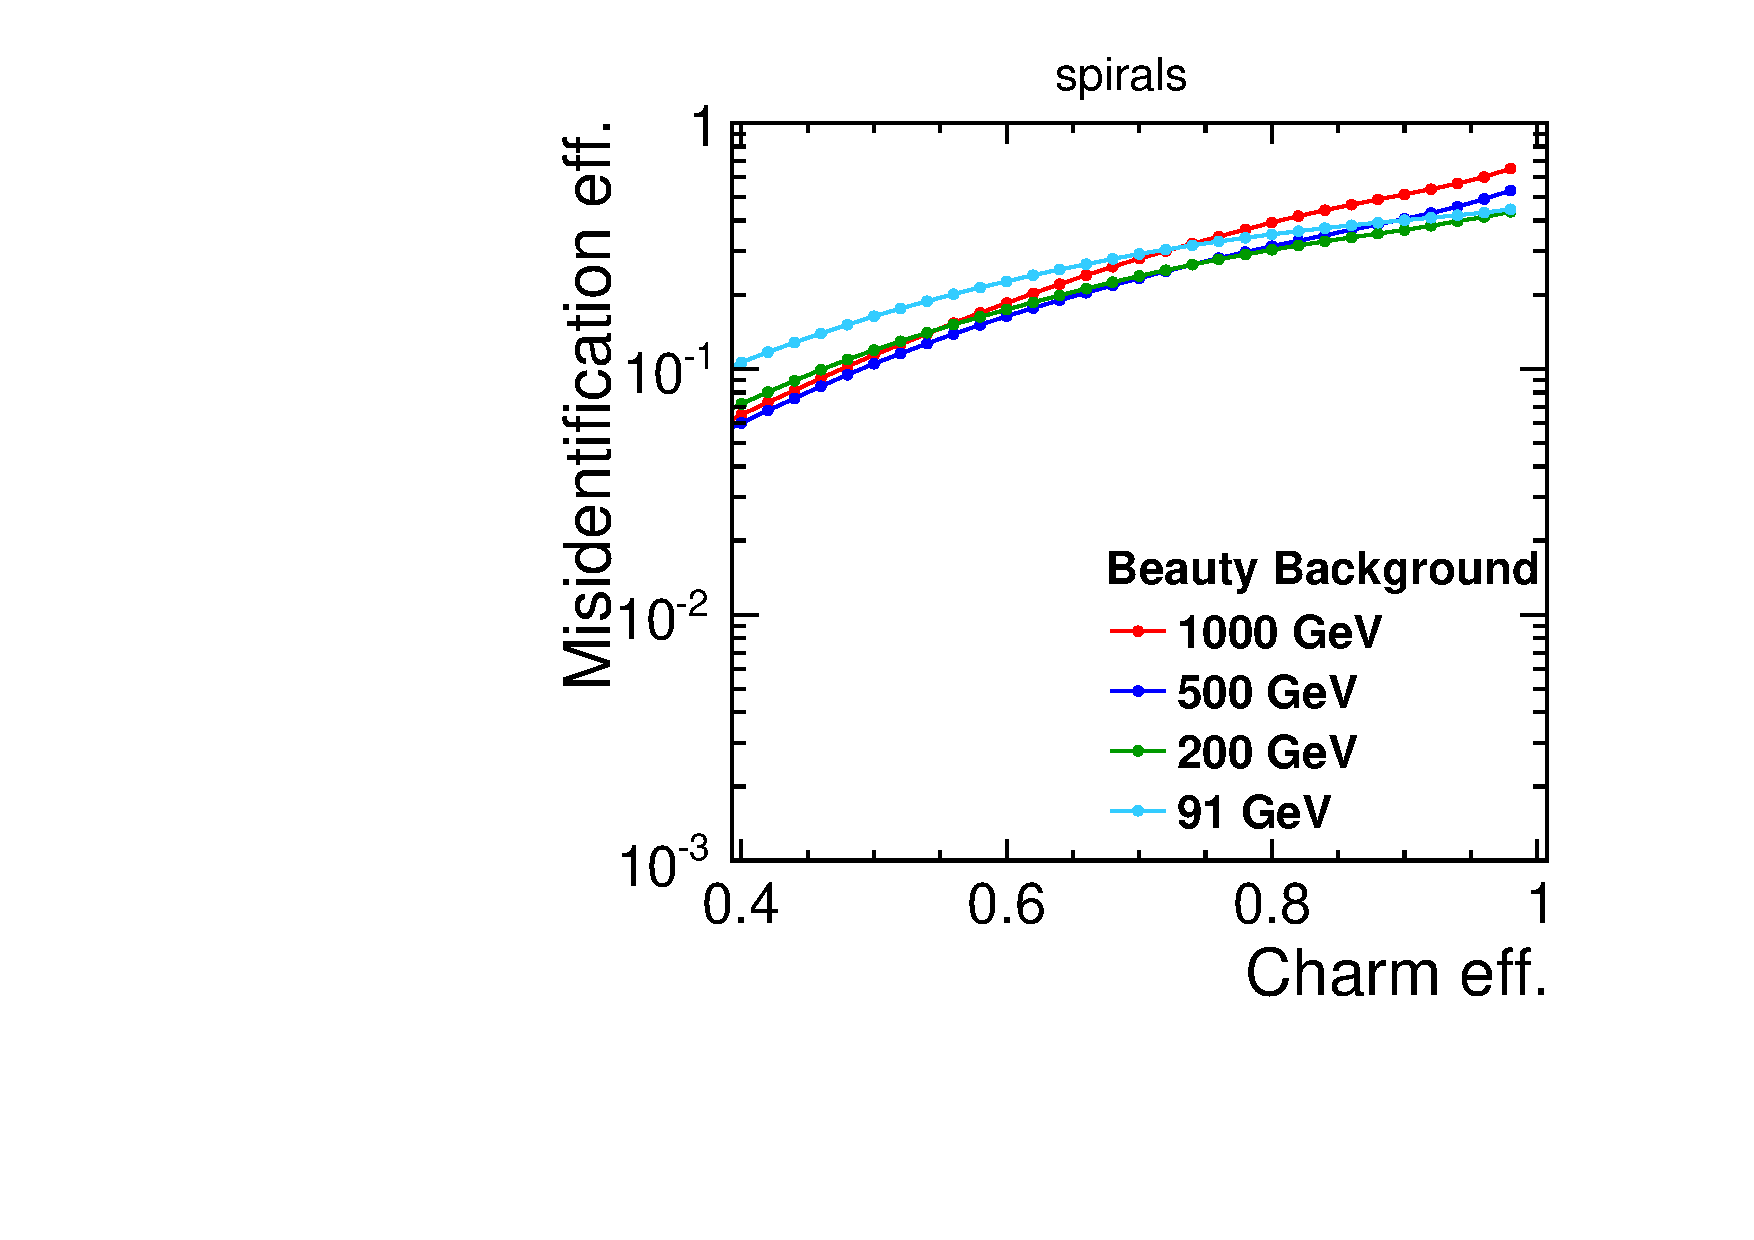
\includegraphics[width=\textwidth]{figures/Global_energies_CLIC_SiD_spirals_Charm_Beauty_.pdf}
  \end{columns}

\end{frame}


%%%%%%%%%%%%%%%%%%%%%%%%%%%%%
%         SLIDE             %
%%%%%%%%%%%%%%%%%%%%%%%%%%%%%
\begin{frame}
  \frametitle{R\&D for pixel detectors at CLIC}

  \begin{columns}
    \column{0.6\textwidth}
    \begin{itemize}
    \item Achieve $3\,\micron$ single-point resolution with:
      \begin{itemize}
      \item Low material: $50\,\micron$-thick sensor on
        $50\,\micron$-thick ASIC. 
      \item Small pitch: $25\,\micron$ pixel pitch.
      \end{itemize}
    \end{itemize}

    \column{0.4\textwidth}
    \centering
    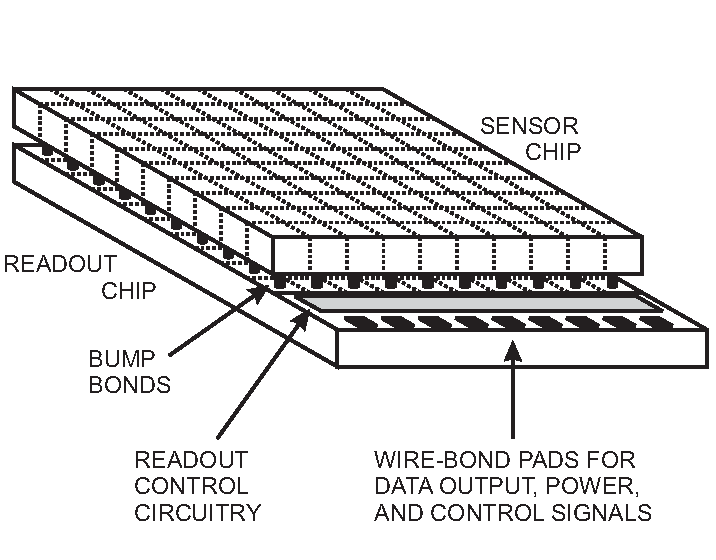
\includegraphics[width=\textwidth]{figures/hybridDet.pdf}
  \end{columns}

  \begin{itemize}
  \item Thin-sensors R\&D:
    \begin{itemize}
    \item The feasibility of thin sensors studied using the Timepix3
      readout ASIC with \textcolor{Red}{$55\,\micron$} pixel pitch.
    \item Use simulations to extrapolate to pixels with a pitch of
      \textcolor{Red}{$25\,\micron$}.
    \end{itemize}
  \end{itemize}

  \begin{itemize}
  \item Small-pitch ASIC R\&D:
    \begin{itemize}
    \item CLICpix readout ASIC demonstrator
    \item Matrix of $64\times64$ pixels, $25\,\micron$ pixel pitch.
    \item 65~nm CMOS technology
    \item Simultaneous measurement of time (TOA) and energy (TOT) per
      pixel.
    \item Compatible with power pulsing scheme.
    \end{itemize}
  \end{itemize}

\end{frame}

%%%%%%%%%%%%%%%%%%%%%%%%%%%%%
%         SLIDE             %
%%%%%%%%%%%%%%%%%%%%%%%%%%%%%
\begin{frame}
  \frametitle{Test-beam measurements of thin sensors}

  % \begin{itemize}
  % \end{itemize}

\end{frame}
% %-------------------------------------------------------
% %-------------------------------------------------------
% \section{R\&D on sensor and readout technologies}
% %-------------------------------------------------------
% \subsection{Thin planar sensors}
% \begin{frame}
%   \frametitle{Thin planar sensors}
% \end{frame}
% %-------------------------------------------------------
% \subsection{The Timepix3 hybrid readout ASIC}
% \begin{frame}
%   \frametitle{The Timepix3 hybrid readout ASICs}
% \end{frame}
% %-------------------------------------------------------
% \begin{frame}
%   \frametitle{Assembly calibration}
% \end{frame}

% %-------------------------------------------------------
% %-------------------------------------------------------
% \section{Simulation}
% \begin{frame}
%   \frametitle{Simulation and reconstruction}
% \end{frame}


% %-------------------------------------------------------
% %-------------------------------------------------------
% \section{Timepix3 beam telescope}
% \begin{frame}
%   \frametitle{Timepix3 beam telescope}
% \end{frame}

% %-------------------------------------------------------
% %-------------------------------------------------------
% \section{Thin sensors studies}
% \begin{frame}
%   \frametitle{Thin sensors studies}
% \end{frame}

% %-------------------------------------------------------
% %-------------------------------------------------------
% \section{Active edge sensors}
% \begin{frame}
%   \frametitle{Active edge sensors}
% \end{frame}

% %-------------------------------------------------------
% %-------------------------------------------------------
\label{lastslide}
\section{Conclusions}
\begin{frame}
  \frametitle{Conclusions}
\end{frame}